%%%%%%%%%%%%%%%%%%%%%%%%%%%%% Define Article %%%%%%%%%%%%%%%%%%%%%%%%%%%%%%%%%%
\documentclass{article}
%%%%%%%%%%%%%%%%%%%%%%%%%%%%%%%%%%%%%%%%%%%%%%%%%%%%%%%%%%%%%%%%%%%%%%%%%%%%%%%

%%%%%%%%%%%%%%%%%%%%%%%%%%%%% Using Packages %%%%%%%%%%%%%%%%%%%%%%%%%%%%%%%%%%
\usepackage{geometry}
\usepackage{graphicx}
\usepackage{amssymb}
\usepackage{amsmath}
\usepackage{amsthm}
\usepackage{empheq}
\usepackage{mdframed}
\usepackage{booktabs}
\usepackage{lipsum}
\usepackage{graphicx}
\usepackage{color}
\usepackage{psfrag}
\usepackage{pgfplots}
\usepackage{bm}
\usepackage{listings}
\usepackage[utf8]{inputenc}
\usepackage{hyperref}
\usepackage{graphicx}

%%%%%%%%%%%%%%%%%%%%%%%%%%%%%%%%%%%%%%%%%%%%%%%%%%%%%%%%%%%%%%%%%%%%%%%%%%%%%%%

% Other Settings

%%%%%%%%%%%%%%%%%%%%%%%%%% Page Setting %%%%%%%%%%%%%%%%%%%%%%%%%%%%%%%%%%%%%%%
\geometry{a4paper}

%%%%%%%%%%%%%%%%%%%%%%%%%% Define some useful colors %%%%%%%%%%%%%%%%%%%%%%%%%%
\definecolor{ocre}{RGB}{243,102,25}
\definecolor{mygray}{RGB}{243,243,244}
\definecolor{deepGreen}{RGB}{26,111,0}
\definecolor{shallowGreen}{RGB}{235,255,255}
\definecolor{deepBlue}{RGB}{61,124,222}
\definecolor{shallowBlue}{RGB}{235,249,255}
%%%%%%%%%%%%%%%%%%%%%%%%%%%%%%%%%%%%%%%%%%%%%%%%%%%%%%%%%%%%%%%%%%%%%%%%%%%%%%%

%%%%%%%%%%%%%%%%%%%%%%%%%% Define an orangebox command %%%%%%%%%%%%%%%%%%%%%%%%
\newcommand\orangebox[1]{\fcolorbox{ocre}{mygray}{\hspace{1em}#1\hspace{1em}}}
%%%%%%%%%%%%%%%%%%%%%%%%%%%%%%%%%%%%%%%%%%%%%%%%%%%%%%%%%%%%%%%%%%%%%%%%%%%%%%%

%%%%%%%%%%%%%%%%%%%%%%%%%%%% English Environments %%%%%%%%%%%%%%%%%%%%%%%%%%%%%
\newtheoremstyle{mytheoremstyle}{3pt}{3pt}{\normalfont}{0cm}{\rmfamily\bfseries}{}{1em}{{\color{black}\thmname{#1}~\thmnumber{#2}}\thmnote{\,--\,#3}}
\newtheoremstyle{myproblemstyle}{3pt}{3pt}{\normalfont}{0cm}{\rmfamily\bfseries}{}{1em}{{\color{black}\thmname{#1}~\thmnumber{#2}}\thmnote{\,--\,#3}}
\theoremstyle{mytheoremstyle}
\newmdtheoremenv[linewidth=1pt,backgroundcolor=shallowGreen,linecolor=deepGreen,leftmargin=0pt,innerleftmargin=20pt,innerrightmargin=20pt,]{theorem}{Theorem}[section]
\theoremstyle{mytheoremstyle}
\newmdtheoremenv[linewidth=1pt,backgroundcolor=shallowBlue,linecolor=deepBlue,leftmargin=0pt,innerleftmargin=20pt,innerrightmargin=20pt,]{definition}{Definition}[section]
\theoremstyle{myproblemstyle}
\newmdtheoremenv[linecolor=black,leftmargin=0pt,innerleftmargin=10pt,innerrightmargin=10pt,]{problem}{Problem}[section]
%%%%%%%%%%%%%%%%%%%%%%%%%%%%%%%%%%%%%%%%%%%%%%%%%%%%%%%%%%%%%%%%%%%%%%%%%%%%%%%

%%%%%%%%%%%%%%%%%%%%%%%%%%%%%%% Plotting Settings %%%%%%%%%%%%%%%%%%%%%%%%%%%%%
\usepgfplotslibrary{colorbrewer}
\pgfplotsset{width=8cm,compat=1.9}
%%%%%%%%%%%%%%%%%%%%%%%%%%%%%%%%%%%%%%%%%%%%%%%%%%%%%%%%%%%%%%%%%%%%%%%%%%%%%%%

%%%%%%%%%%%%%%%%%%%%%%%%%%%%%%% Title & Author %%%%%%%%%%%%%%%%%%%%%%%%%%%%%%%%
\title{La importancia de las matrices en la inteligencia artificial.}
\author{Alejandro Gutiérrez Grimaldo}
%%%%%%%%%%%%%%%%%%%%%%%%%%%%%%%%%%%%%%%%%%%%%%%%%%%%%%%%%%%%%%%%%%%%%%%%%%%%%%%

\begin{document}
    \maketitle
\section{Introducción}

Objetivo: Dar una introducción de cómo funciona la inteligencia artificial, enfocado en el uso de matrices para el aprendizaje de esta (Machine Learning). Al igual que varios conceptos técnicos especializados en esta rama de la ingeniería en computación.
\\
\\
En esta investigación se presentan las aplicaciones de las matrices en la inteligencia artificial, desde el procesamiento del lenguaje natural y el aprendizaje automático hasta el análisis de datos, la teoría de grafos, la simulación y modelado, la inteligencia distribuida y en tiempo real y nuevas tecnologías como la inteligencia cuántica.
\\
\\
He visto cómo las matrices son esenciales en la inteligencia artificial, ya que permiten representar y manipular datos de manera eficiente. He aprendido cómo se crean matrices en Python utilizando la librería NumPy, y cómo se utilizan en tareas de aprendizaje automático y procesamiento de datos.
\\
\\
También cómo las matrices son utilizadas en el proceso de optimización y en la resolución de problemas de optimización, ilustrando con un ejemplo práctico de entrenamiento de una red neuronal con el conjunto de datos MNIST y con la librería Keras.
\\
\\
Es importante señalar que esta investigación es solo una introducción a este tema y hay mucho más por aprender y explorar sobre el uso de matrices en la inteligencia artificial. Los conceptos y ejemplos presentados aquí son solo una pequeña muestra de las posibilidades que ofrecen las matrices en la Inteligencia Artificial y es importante continuar estudiando para aprender más sobre estas herramientas.


\section{Desarrollo}

La inteligencia artificial según el diccionario es: “Disciplina científica que se ocupa de crear programas informáticos que ejecutan operaciones comparables a las que realiza la mente humana, como el aprendizaje o el razonamiento lógico.” (RAE, 2022). Aunque la implementación de la inteligencia artificial en la cotidianidad es un tema muy interesante, voy a profundizar en términos más técnicos y relacionado a las matemáticas utilizadas en esta tecnología, para ser específico, en las matrices.
\\
\\
Existen varios usos importantes de las matrices en la inteligencia artificial. Uno de ellos es en el procesamiento del lenguaje natural, donde las matrices son utilizadas para representar palabras y frases en forma de vectores, lo que permite realizar tareas como la clasificación y la predicción de texto.
\\
\\
En el aprendizaje automático, las matrices también son fundamentales. Se utilizan para representar y optimizar modelos de machine learning, como redes neuronales. En el entrenamiento de estas redes, las matrices son utilizadas para representar los pesos y los sesgos de las conexiones entre las neuronas, así como para calcular los gradientes en el proceso de optimización.
\\
\\
Otra área importante donde se utilizan las matrices es en la resolución de problemas de optimización. Por ejemplo, en el aprendizaje por refuerzo, las matrices son utilizadas para representar el estado de un entorno y para calcular la acción óptima a tomar en cada paso.
Además, las matrices también son utilizadas en áreas como la visión artificial y el procesamiento de imágenes, donde son utilizadas para representar y procesar datos de imágenes en forma de matrices de píxeles.
\\
\\
Además, las matrices también son utilizadas en técnicas de procesamiento de señales y sistemas dinámicos, como en el control automático y la robótica, para modelar y controlar sistemas complejos.
\\
\\
En el campo del aprendizaje automático, las matrices son esenciales en el uso de algoritmos de aprendizaje supervisado y no supervisado. 

\begin{itemize}
    \item Aprendizaje supervisado: Las matrices son utilizadas para representar los datos de entrenamiento y las etiquetas correspondientes.
    \item Aprendizaje no supervisado: se utilizan las matrices para representar los datos y encontrar patrones o estructuras ocultas en ellos.
\end{itemize}
\parskip 0.5em
Además, las matrices son muy útiles en algoritmos de procesamiento de datos masivos, como el procesamiento de datos distribuidos[1] y el procesamiento de datos en paralelo[2], ya que permite la distribución eficiente de los datos y la paralelización de operaciones matriciales para mejorar el rendimiento.
\\
\\
Además de las aplicaciones mencionadas anteriormente, las matrices también tienen un papel importante en el ámbito del análisis de datos. Por ejemplo, en el análisis de componentes principales[3] (Principal Component Analysis, PCA) y la factorización de matrices, se utilizan matrices para representar los datos y encontrar patrones ocultos en ellos, lo que ayuda a comprender mejor y visualizar los datos.
\\
\\
Otra aplicación importante de las matrices en el análisis de datos es en la recomendación de sistemas, donde se utilizan para representar los datos de usuarios y productos, y para calcular las similitudes entre ellos. Esto permite la recomendación de productos o contenido personalizado a los usuarios.
\\
\\
En el campo del aprendizaje automático, las matrices también son esenciales en la utilización de algoritmos de deep learning , como las redes neuronales profundas[4] (Deep Neural Networks, DNNs) y las redes neuronales convolucionales[5] (Convolutional Neural Networks,CNNs). En estos algoritmos, las matrices son utilizadas para representar los datos de entrada y los pesos de las conexiones entre las neuronas. Además, también son utilizadas en el entrenamiento de estos modelos mediante el uso de técnicas de optimización como el gradiente descendente.
\\
\\
Otra aplicación importante de las matrices en la inteligencia artificial es en el campo de la teoría de grafos[6]. Las matrices de adyacencia y la matriz de incidencia se utilizan para representar grafos y su estructura, permitiendo el análisis de patrones y relaciones en los mismos.
\\
\\
En el campo de la recuperación de información, las matrices son utilizadas para representar los datos de los documentos y las consultas, permitiendo la búsqueda de información relevante en grandes cantidades de datos.
\\
\\
Las matrices también son útiles en el campo de la simulación y modelado, donde se utilizan para representar sistemas físicos y modelos matemáticos. Esto permite simular y predecir el comportamiento de los sistemas a través del tiempo, lo que es esencial en aplicaciones como la simulación de procesos químicos y la predicción del clima.
\\
\\
En el campo de la inteligencia computacional distribuida, las matrices también tienen un papel importante. Un ejemplo es el uso de matrices distribuidas en clusters y sistemas distribuidos, que permite la paralelización y distribución de cálculos matriciales, lo que mejora el rendimiento en el procesamiento de grandes volúmenes de datos.
\\
\\
En el campo de la inteligencia artificial en tiempo real, las matrices también son esenciales. Por ejemplo, en sistemas de control en tiempo real y en sistemas de seguimiento y rastreo, las matrices son utilizadas para modelar y controlar sistemas en tiempo real, lo que permite una toma de decisiones rápida y precisa.
\\
\\
Finalmente, también están surgiendo nuevas aplicaciones y tecnologías en las que las matrices juegan un papel importante. Por ejemplo, en el campo de la inteligencia cuántica[7], las matrices se utilizan para representar estados cuánticos y para desarrollar algoritmos cuánticos.

\subsection{Ejemplos prácticos.}

Requerimientos:

\begin{itemize}
    \item Computadora con internet.
    \item IDE (Yo utilize Visual Studio Code, puedes ocupar el de tu preferencia).
    \item Acceso a la terminal (En mi caso use PowerShell).
    \item SDK de Python con pip para la instalación de librerías (numpy, keras).
    \end{itemize}

Enlaces de descarga.

\subsection{Introducción a los ejemplos}

En este proyecto, vamos a utilizar el lenguaje de programación Python para ilustrar cómo se utilizan las matrices en la inteligencia artificial. Python es un lenguaje de programación de alto nivel y fácil de aprender, con una amplia variedad de librerías y paquetes que hacen que sea ideal para el desarrollo de proyectos de aprendizaje automático y procesamiento de datos.

En particular, vamos a utilizar la librería NumPy, que proporciona una amplia variedad de funciones y operaciones matriciales, así como también una implementación eficiente de las matrices en Python. También podremos utilizar otras librerías como SciPy o scikit-learn para ilustrar algoritmos y técnicas de aprendizaje automático.

A medida que avanzamos en este proyecto, aprenderemos cómo crear y manipular matrices en Python, así como cómo utilizarlas en tareas de aprendizaje automático y procesamiento de datos. También veremos cómo las matrices son esenciales en el proceso de optimización y en la resolución de problemas de optimización. En resumen, este ejemplo es una introducción al uso de matrices en la inteligencia artificial y al mismo tiempo un tutorial de programación en Python.

\subsection{Desarrollo}

\subsubsection{Ejemplo 1}

Existen varias formas de crear matrices en Python utilizando la librería NumPy. A continuación muestro algunos ejemplos:
\\
\\
En primera instancia tenemos que instalar la biblioteca requerida con el comando pip install numpy.

\begin{figure}[ht]
    \centering
    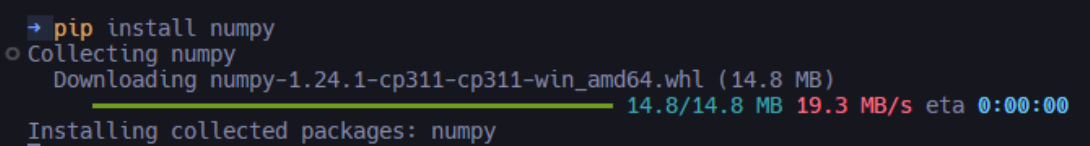
\includegraphics[width=0.8\textwidth]{terminal1.png}
    \caption{Instalación de la biblioteca numpy con la terminal}
    \label{fig:1}
\end{figure}

\begin{lstlisting}[language=Python]
    import numpy as np

    # Crear una matriz para representar los datos de entrenamiento
    X = np.array([[1, 2], [3, 4], [5, 6]])
    y = np.array([7, 8, 9])
    
    # Crear una matriz para almacenar los pesos
    w = np.array([0, 0])
    
    # Realizar una regresion lineal simple
    for i in range(1000):
        y_pred = X.dot(w)
        error = y_pred - y
        grad = X.T.dot(error) / len(X)
        w -= 0.01 * grad
    
    print(w)
    
    
\end{lstlisting}
Estas son las formas más comunes para introducir una matriz en python con la librería numpy.

\subsubsection{Ejemplo 2}

En este ejemplo, vamos a utilizar una matriz para representar un conjunto de datos de entrenamiento y otra para realizar una regresión lineal simple:

\begin{lstlisting}[language=Python]
    import numpy as np
    #crear una matriz vacia:
    A = np.array([])
    #crear una matriz a partir de una lista:
    B = np.array([[1, 2, 3], [4, 5, 6], [7, 8, 9]])
    #Crear una matriz llena de ceros o unos:
    C = np.zeros((3, 3))
    D = np.ones((3, 3))
    #Crear una matriz con un valor especifico:
    E = np.full((3, 3), 7)
    #Crear una matriz identidad:
    F = np.eye(3)
    #Crear una matriz con valores aleatorios:
    G = np.random.rand(3, 3)
    H = np.random.randn(3, 3)
    #Crear una matriz a partir de una secuencia:
    I = np.arange(0, 9).reshape(3,3)
\end{lstlisting}

\subsubsection{Ejemplo 3}

En este ejemplo, se utiliza la librería Keras para crear una red neuronal simple para clasificar imágenes. Se instala con el comando ‘pip install keras’.

\begin{figure}[ht]
    \centering
    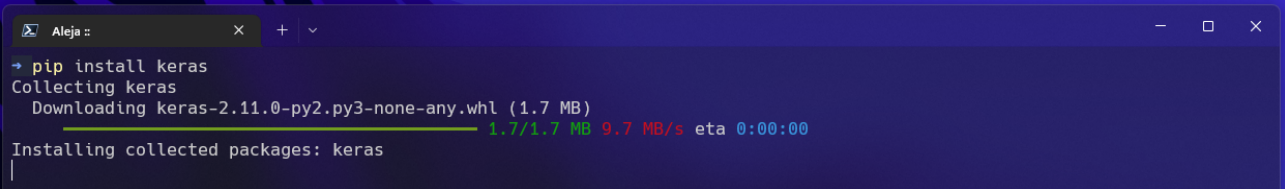
\includegraphics[width=0.9\textwidth]{terminal2.png}
    \caption{ Instalación de keras con la terminal}
    \label{fig:2}
\end{figure}
\parskip 0.5em
En este ejemplo, primero creamos una matriz de numpy llamada "X" para representar nuestros datos de entrenamiento, con 3 ejemplos y 2 características. Luego creamos otra matriz llamada "y" para almacenar las etiquetas correspondientes. A continuación, creamos una matriz llamada "w" para almacenar los pesos de nuestro modelo.
\\
\\
En el bucle, utilizamos la función "dot" de numpy para realizar el producto matricial entre X y W, lo que nos da las predicciones de nuestro modelo. Luego calculamos el error como la diferencia entre las predicciones y las etiquetas reales.
\\
\\
Finalmente, calculamos el gradiente utilizando la transpuesta de X y el error y actualizamos los pesos del modelo mediante un proceso de optimización mediante gradiente descente. Al finalizar el bucle, imprimimos los pesos del modelo, que son los parámetros aprendidos a partir de los datos de entrenamiento.
\\
\\
Este ejemplo es simplificado con fines educativos y está regresión lineal es muy sencilla. En general se recomienda usar librerías y paquetes que implementan algoritmos más complejos y con mejor rendimiento.
\\
\\
En este ejemplo, se utiliza la librería Keras para crear una red neuronal simple para clasificar imágenes. Se instala con el comando pip install keras.
\parskip 0.5em
\\
\\
Primero, se cargan los datos de entrenamiento y prueba del conjunto de datos MNIST utilizando la función de carga de datos de Keras. Luego, se normalizan los datos y se convierten en una matriz con un vector de 784 elementos para aplanar las imágenes. A continuación, se utiliza la función to categorical de Keras para convertir las etiquetas en categorías.
\\
\\
Después se define un modelo secuencial, una serie de capas conectadas secuencialmente, que agrega dos capas densas (capa completamente conectadas) a la red neuronal. La primera capa tiene 512 unidades y una función de activación relu, y la segunda capa tiene 10 unidades y una función de activación softmax.
\\
\\
Finalmente, se compila el modelo, se especifican los parámetros de optimización y la función de pérdida, y se entrena el modelo utilizando los datos de entrenamiento y las etiquetas correspondientes.
\\
\\
Esto es solo un ejemplo simplificado de cómo se podría hacer. Es importante considerar que en un proyecto real se deben considerar otros factores, como la validación cruzada, el ajuste de hiperparámetros, entre otros.
\\
\section{Conclusión.}

Como bien mencione en el proyecto, las matrices en ingeniería en computación y principalmente en la inteligencia artificial es extremadamente fundamental, desde el mismo procesamiento de datos, como son evaluados y la eficiencia de los recursos disponibles. Aunque este tema es extremadamente extenso y me hubiera gustado incluir más acerca de Big Data, los entrenamientos y la implementación de estas inteligencias artificiales, creo que fue una buena introducción en este campo. 
\\
\\
Por más que se piense que la inteligencia artificial está lejos de ser cotidiana, solo hace falta ver a nuestro alrededor, en nuestro teléfono tenemos bastantes, desde un asistente de voz, inteligencias que estudian nuestras preferencias en redes sociales, o para la misma conducción autónoma de algunos coches.
\\
\\
Las matemáticas han sido y serán un pilar en la tecnología, porque es la mejor manera de predecir lo que puede pasar, este fue un ejemplo con matrices, pero hay más campos donde las matrices juegan un papel importante, así como también donde las inteligencias artificiales requieren otros métodos matemáticos.
\\
\\
Por lo tanto, lector o lectora, te invito a que sigas profundizando en el conocimiento de estas tecnologías, ya que van a ser de gran importancia para los avances tecnológicos de un futuro cercano.
\section{Glosario.}
\begin{itemize}
    
    \item [1]Procesamiento de datos distribuidos: Son un conjunto de datos que están divididos en varias partes y almacenados en diferentes lugares, ya sea en diferentes servidores, máquinas, dispositivos o redes; las herramientas que usan esta tecnología son: Hadoop HDFS, Apache Cassandra, MongoDB, y Apache Kafka.
    \item [2]Procesamiento de datos en paralelo: Es una técnica de procesamiento en la cual se dividen los datos en varias partes y se procesan simultáneamente en diferentes unidades de procesamiento, como múltiples núcleos de un procesador, varios procesadores en una computadora o varias computadoras en una red, las herramientas que usan esta tecnología son: OpenMP, MPI y CUDA.
    \item [3]Análisis de componentes principales: es un método estadístico utilizado para analizar y reducir la dimensión de un conjunto de datos. El objetivo principal de PCA es encontrar un conjunto de componentes principales que expliquen la mayor cantidad de varianza en los datos, y que sean ortogonales entre sí. Para realizar un PCA en un conjunto de datos se sigue los siguientes pasos:
    \begin{itemize}
        \item Calcular la matriz de covarianza.
        \item Calcular los autovectores y autovalores de la matriz de covarianza.
        \item Seleccionar los componentes principales.
        \item Proyectar los datos en el subespacio de menor dimensión.
    \end{itemize}
    \item [4]Redes neuronales profundas: Hay varias capas de neuronas, lo que permite a la red aprender representaciones cada vez más complejas de los datos a medida que se procesan a través de las capas.
    \item [5]Redes neuronales convolucionales: Se caracterizan por tener capas de convolución y pooling que les permiten aprender patrones y características específicas de los datos de imagen.
    \item [6]Teoría de grafos: Son estructuras matemáticas formadas por un conjunto de vértices o nodos, y un conjunto de arcos o enlaces que los conectan. Los grafos se utilizan para representar relaciones entre objetos o entidades, y son útiles para modelar problemas en una gran variedad de campos, incluyendo la teoría de redes, la teoría de la computación, la inteligencia artificial, la teoría de sistemas y la teoría de sistemas dinámicos.
    \item [7]Inteligencia cuántica: La inteligencia cuántica se refiere al uso de la mecánica cuántica para desarrollar algoritmos y técnicas de inteligencia artificial. La mecánica cuántica es una teoría física que describe el comportamiento de la materia y la energía a nivel subatómico, y se caracteriza por la superposición, el entrelazamiento y la no-localidad. La inteligencia cuántica se diferencia de la inteligencia artificial tradicional, que se basa en técnicas y algoritmos clásicos, ya que aprovecha las propiedades cuánticas para desarrollar algoritmos y técnicas más eficientes.
\end{itemize}
\section{Enlaces de descarga.}
\begin{itemize}
    \item \href{https://www.python.org/downloads/}{SDK de Python}
    \item \href{https://code.visualstudio.com/}{Visual Studio Code}
    \item \href{https://apps.microsoft.com/store/detail/powershell/}{PowerShell}
    \item pip install numpy
    \item pip install keras
\end{itemize}

\section{Fuentes.}
{Derivando2021,
  title={¿Qué es y cómo funciona la INTELIGENCIA ARTIFICIAL?},
  author={Derivando},
  year={2021},
  url={https://www.youtube.com/watch},
  note={YouTube Video},
}

{Mike2019,
  title={Array Basics},
  author={Mike},
  year={2019},
  month={Dec},
  url={https://www.machinelearningmike.com/post/array-basics},
}

{Kwiatkowski2018,
  title={Machine Learning From Scratch: Part 3 - Towards Data Science},
  author={Kwiatkowski, S.},
  year={2018},
  month={Mar},
  url={https://towardsdatascience.com/machine-learning-from-scratch-part-3-ed572330367d},
  note={Medium; Towards Data Science},
}

{Nimbalkar2021,
  title={Artificial Intelligence Machine Learning Arrays — Perfect team},
  author={Nimbalkar, R.},
  year={2021},
  month={Jun},
  url={https://medium.com/appengine-ai/artificial-intelligence-machine-learning-arrays-perfect-team-293b22474c91},
  note={Medium; appengine.ai},
}

{NumPyDocs2022,
  title={NumPy documentation - NumPy v1.24 Manual},
  author={NumPy},
  year={2022},
  url={https://numpy.org/doc/stable/},
}

{IASolver2021,
  title={6 Librerías imprescindibles de Python para Machine Learning},
  author={IA SOLVER},
  year={2021},
  month={Jun},
  url={https://iasolver.es/6-librerias-de-python-para-machine-learning},
}

{Bustos2021,
  title={Introducción a NumPy de Python},
  author={Bustos, L. R.},
  year={2021},
  month={Jul},
  url={https://www.ciiia.mx/noticiasciiia/introduccin-a-numpy-de-python},
  note={Lic. Luis Roberto Bustos Vargas},
}
{Palo2021,
title={NumPy Tutorial: Your First Steps Into Data Science in Python},
author={Palo, R.},
year={2021},
month={Jan},
day={11},
url={https://realpython.com/numpy-tutorial},
note={Obtenido de Real Python}
}

{Oracle2014,
title={¿Qué es la inteligencia artificial?},
author={Oracle},
year={2014},
url={https://www.oracle.com/mx/artificial-intelligence/what-is-ai/},
}

{Rojas2022,
title={Qué es y cómo funciona la Inteligencia Artificial},
author={Rojas, J.},
year={2022},
month={Nov},
day={25},
url={https://www.telefonica.com/es/sala-comunicacion/blog/que-es-y-como-funciona-la-inteligencia-artificial},
note={Telefónica}
}

{GoogleCloud2023,
title={¿Qué es la inteligencia artificial o IA?},
author={Google Cloud},
year={2023},
url={https://cloud.google.com/learn/what-is-artificial-intelligence?hl=es-419},
}

{MicrosoftAzure2023,
title={¿Qué es la inteligencia artificial?},
author={Microsoft Azure},
year={2023},
url={https://azure.microsoft.com/es-es/resources/cloud-computing-dictionary/what-is-artificial-intelligence/},
}

{binMohamed2022,
title={Artificial intelligence in mathematics education: A systematic literature review},
author={bin Mohamed, M. Z. and Hidayat, R. and binti Suhaizi, N. N. and bin Mahmud, M. K. H. and binti Baharuddin, S. N.},
journal={International Electronic Journal of Mathematics Education},
volume={17},
number={3},
pages={em0694},
year={2022},
}

{Deo2020,
title={Modern artificial intelligence model development for undergraduate student performance prediction: An investigation on engineering mathematics courses},
author={Deo, R. C. and Yaseen, Z. M. and Al-Ansari, N. and Nguyen-Huy, T. and Langlands, T. A. M. and Galligan, L.},
journal={IEEE Access},
volume={8},
pages={136697-136724},
year={2020},
}

{Allamanis2018,
title={A survey of machine learning for big code and naturalness},
author={Allamanis, M. and Barr, E. T. and Devanbu, P. and Sutton, C.},
journal={ACM Computing Surveys (CSUR)},
volume={51},
number={4},
pages={1-37},
year={2018},
}

{QuantumIntelligence2022,
title={Quantum Intelligence},
author={Quantum Intelligence},
year={2022},
url={https://quantumintelligence.com/},
}
\end{document}